% ==========================================
% step01.tex
% ==========================================
\section{بخش اول: بهبود کیفیت تصویر به کمک عملگر نقطه‌ای خطی ($I+b$)}

\noindent
عملگر نقطه‌ایِ $I' = I + b$، کل توزیع هیستوگرام تصویر را بدون تغییر در شکل هندسی و پراکندگی آن، به اندازه‌ی $b$ در محور شدت روشنایی جابه‌جا می‌کند ($\mu'=\mu+b$). در این بخش، تأثیر این عملگر بر روی دو تصویر \texttt{BrightImage} (دارای مشکل بیش‌نوردهی یا \lr{Over-exposure}) و \texttt{DarkImage} (دارای مشکل کم‌نوردهی یا \lr{Under-exposure}) با استفاده از مقادیر ثابت و سپس شیفت تطبیقی بهینه مورد ارزیابی قرار می‌گیرد.

\begin{stepbox}
\field{۱. تحلیل توزیع شدت روشنایی در تصاویر ورودی}{
بررسی هیستوگرام تصاویر نشان می‌دهد که پیکسل‌های \texttt{BrightImage} به‌شدت به سمت کران بالای بازه (مقدار $255$) متمایل هستند، درحالی‌که هیستوگرام \texttt{DarkImage} تجمعی فشرده حول مقادیر نزدیک به صفر دارد. هر دو تصویر با فرمت ۸ بیتی بدون علامت (\texttt{uint8}) در بازه‌ی $[0, 255]$ بارگذاری و پردازش شده‌اند.
}
\end{stepbox}

\begin{figure}[htbp]
\centering
\begin{subfigure}{0.48\textwidth}
    \centering
    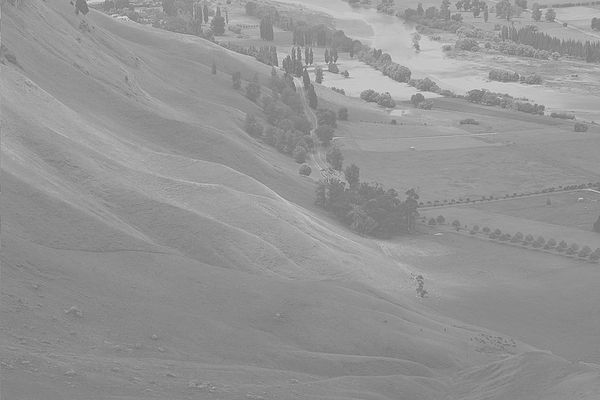
\includegraphics[width=0.85\linewidth]{images/BrightImage.jpg}
    \caption{تصویر \texttt{BrightImage} (بیش‌نوردهی)}
\end{subfigure}
\hfill
\begin{subfigure}{0.48\textwidth}
    \centering
    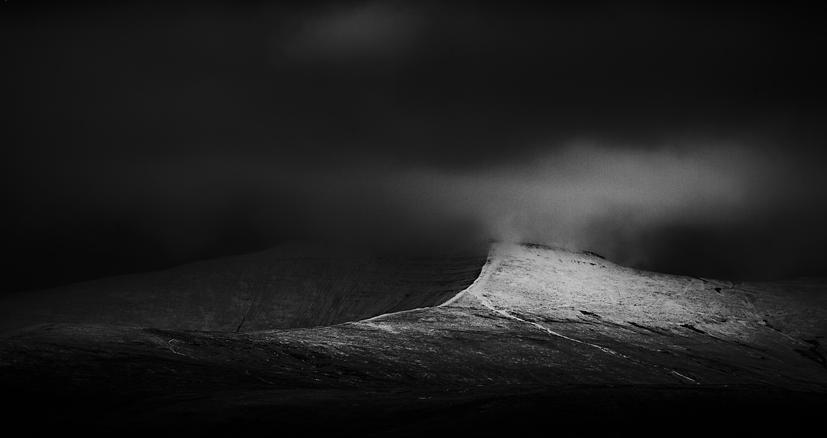
\includegraphics[width=0.85\linewidth]{images/DarkImage.jpg}
    \caption{تصویر \texttt{DarkImage} (کم‌نوردهی)}
\end{subfigure}
\caption{تصاویر خام ورودی پیش از اعمال عملگرهای نقطه‌ای}
\label{fig:originals}
\end{figure}

\begin{stepbox}
\field{۲. اعمال شیفت‌های ثابت $b \in \{-40, -20, +20, +40\}$ و تحلیل خروجی‌ها}{
\textbf{تصویر \texttt{BrightImage}:} افزودن مقادیر مثبت ($I+20$ و $I+40$) منجر به برخورد پیکسل‌ها با سقف بازه و بروز پدیده‌ی \lr{Clipping} شدید می‌شود که حاصل آن، از بین رفتن کامل بافت‌های تصویر در نواحی روشن است. در مقابل، کاهش روشنایی به احیای کنتراست کمک کرده و در این میان، \textbf{$I-40$} با هدایت هیستوگرام به سمت مقادیر میانی (خاکستری)، مطلوب‌ترین کیفیت بصری را ارائه می‌دهد.

\textbf{تصویر \texttt{DarkImage}:} تفریق مقادیر ثابت ($I-20$ و $I-40$) به دلیل ماهیت حلقوی محاسبات در داده‌های ۸ بیتی (\lr{Modulo 256})، باعث بروز خطای \lr{Underflow} شده و پیکسل‌های تاریک را به نویزهای سفیدسوخته (\lr{False Artifacts}) تبدیل می‌کند. در سوی دیگر، افزودن روشنایی، جزئیات پنهان را آشکار می‌سازد و تصویر \textbf{$I+40$} بالاترین کیفیت بصری را در میان گزینه‌های ثابت به خود اختصاص داده است.
}
\end{stepbox}

\begin{warnbox}[مدیریت خطای سرریز در محاسبات \texttt{NumPy}]
محاسبات مستقیم ریاضی بر روی آرایه‌های \texttt{uint8} در کتابخانه‌ی \texttt{NumPy} دارای رفتار پیمانه‌ای هستند (به عنوان مثال $10 - 40 \equiv 226$). برای جلوگیری از این رفتار مخرب که منجر به تخریب تصویر می‌شود، آرایه ابتدا باید به \texttt{int16} تبدیل (\lr{Cast}) شده، پس از اعمال متغیر $b$، مقادیر توسط تابع \texttt{np.clip} در بازه استاندارد $[0, 255]$ فشرده شوند و در نهایت به فرمت \texttt{uint8} بازگردانده شوند.
\end{warnbox}

\begin{figure}[htbp]
\centering
\begin{subfigure}{0.24\textwidth}\centering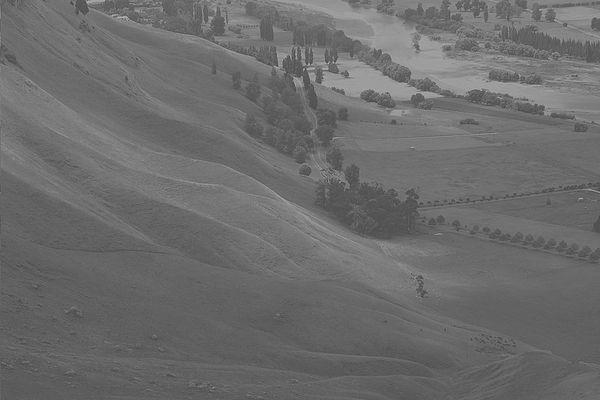
\includegraphics[width=0.95\linewidth]{images/I_BI-40.jpg}\caption{$I - 40$}\end{subfigure}\hfill
\begin{subfigure}{0.24\textwidth}\centering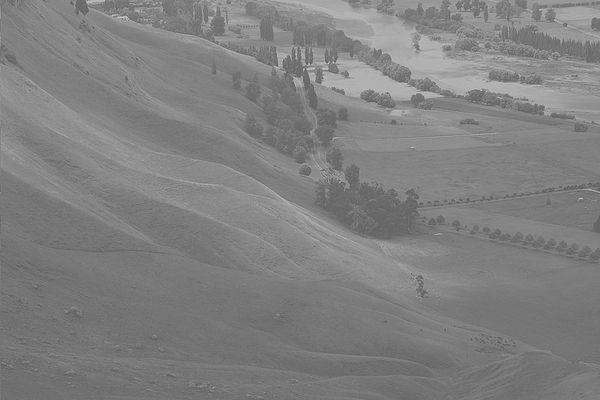
\includegraphics[width=0.95\linewidth]{images/I_BI-20.jpg}\caption{$I - 20$}\end{subfigure}\hfill
\begin{subfigure}{0.24\textwidth}\centering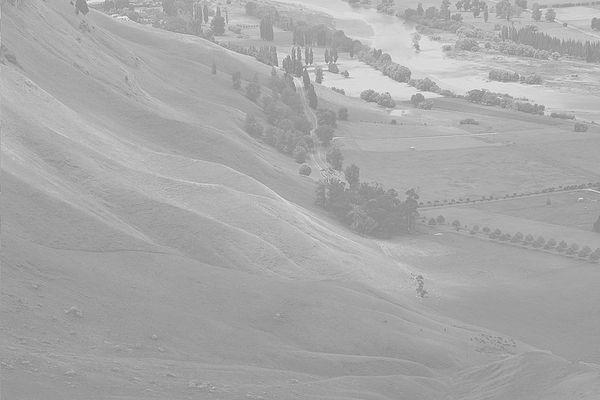
\includegraphics[width=0.95\linewidth]{images/I_BI+20.jpg}\caption{$I + 20$}\end{subfigure}\hfill
\begin{subfigure}{0.24\textwidth}\centering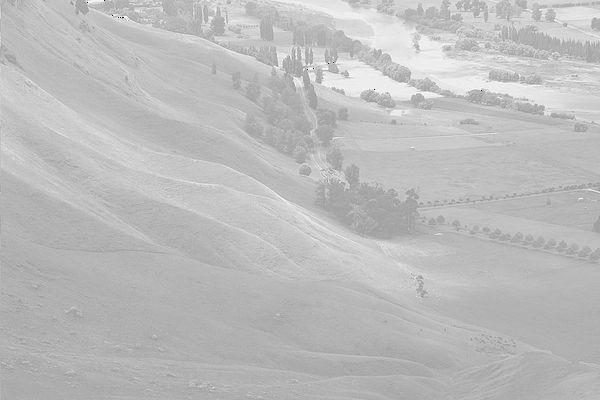
\includegraphics[width=0.95\linewidth]{images/I_BI+40.jpg}\caption{$I + 40$}\end{subfigure}
\caption{تأثیر شیفت‌های ثابت بر روی \texttt{BrightImage} (شاهد از دست رفتن بافت‌ها به دلیل \lr{Clipping} در تصاویر سمت راست هستیم)}
\label{fig:bi_shifts}
\end{figure}

\begin{figure}[htbp]
\centering
\begin{subfigure}{0.24\textwidth}\centering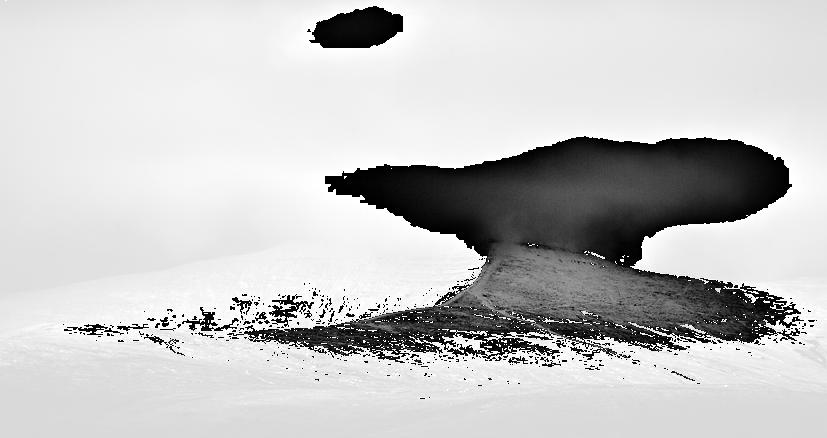
\includegraphics[width=0.95\linewidth]{images/I_DI-40.jpg}\caption{$I - 40$}\end{subfigure}\hfill
\begin{subfigure}{0.24\textwidth}\centering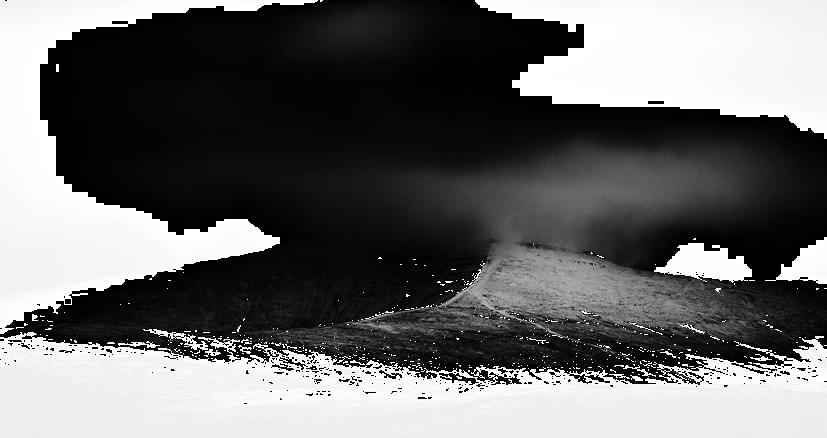
\includegraphics[width=0.95\linewidth]{images/I_DI-20.jpg}\caption{$I - 20$}\end{subfigure}\hfill
\begin{subfigure}{0.24\textwidth}\centering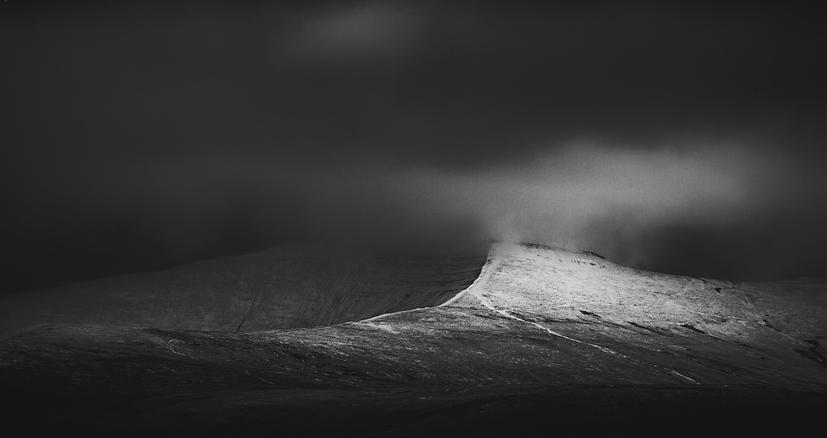
\includegraphics[width=0.95\linewidth]{images/I_DI+20.jpg}\caption{$I + 20$}\end{subfigure}\hfill
\begin{subfigure}{0.24\textwidth}\centering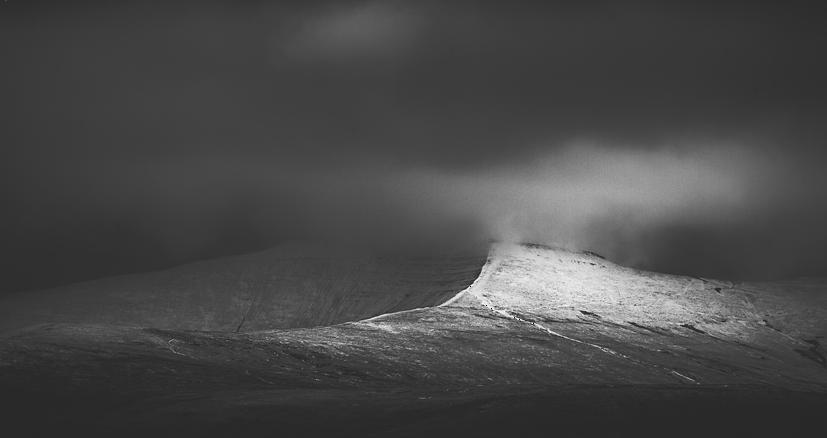
\includegraphics[width=0.95\linewidth]{images/I_DI+40.jpg}\caption{$I + 40$}\end{subfigure}
\caption{تأثیر شیفت‌های ثابت بر روی \texttt{DarkImage} (شاهد بروز اعوجاج و خطای \lr{Underflow} در تصاویر سمت چپ هستیم)}
\label{fig:di_shifts}
\end{figure}

\begin{stepbox}
\field{۳. محاسبه‌ی بایاس بهینه ($b_{opt}$) به‌صورت تطبیقی}{
برای ایجاد یک راه‌حل مستقل از تنظیم دستی، معیار ایده‌آل انتقال ممان اول (میانگین روشنایی، $\mu$) به مرکز بازه‌ی ۸ بیتی (عدد $128$) است؛ یعنی $b_{ideal} = 128 - \mu$. با این وجود، انتقال کامل هیستوگرامِ تصاویری که چولگی شدید دارند، منجر به برخورد پیکسل‌های مرزی با سمت مقابل و فشردگی (\lr{Clipping}) اطلاعات می‌شود. لذا این مقدار پایه با ضرایب تجربی برای هر تصویر تعدیل گردید:
\[
b_{opt}^{DI} = \left\lfloor \frac{128 - \mu_{DI}}{2} \right\rfloor, \qquad b_{opt}^{BI} = 2 \times (128 - \mu_{BI})
\]
برای تصویر تاریک، اعمال ضریب $0.5$ از سفیدسوختگی پس‌زمینه جلوگیری کرده و برای تصویر روشن، ضریب $2$ باعث شیفت کافی بافت‌های خاکستری به سمت تیرگیِ مطلوب می‌شود.
}
\end{stepbox}

\begin{codebox}[الگوریتم محاسبه بایاس بهینه و مدیریت بازه]
\begin{lstlisting}[language=Python]
# --- Optimal Bias for DarkImage ---
mean_val_DI = int(I_DI.flatten().mean())
b_DI_opt = (128 - mean_val_DI) // 2
new_image_DI = np.clip(I_DI.astype(np.int16) + b_DI_opt, 0, 255).astype(np.uint8)

# --- Optimal Bias for BrightImage ---
mean_val_BI = int(I_BI.flatten().mean())
b_BI_opt = (128 - mean_val_BI) * 2
new_image_BI = np.clip(I_BI.astype(np.int16) + b_BI_opt, 0, 255).astype(np.uint8)
\end{lstlisting}
\end{codebox}

\begin{figure}[htbp]
\centering
% سطر اول: تصویر و هیستوگرام تاریک
\begin{subfigure}{0.48\textwidth}
    \centering
    
\includegraphics[width=0.85\linewidth]{images/I_DI+b_DI.jpg}
    \caption{تصویر \texttt{DarkImage} بهینه‌شده}
\end{subfigure}
\hfill
\begin{subfigure}{0.48\textwidth}
    \centering
    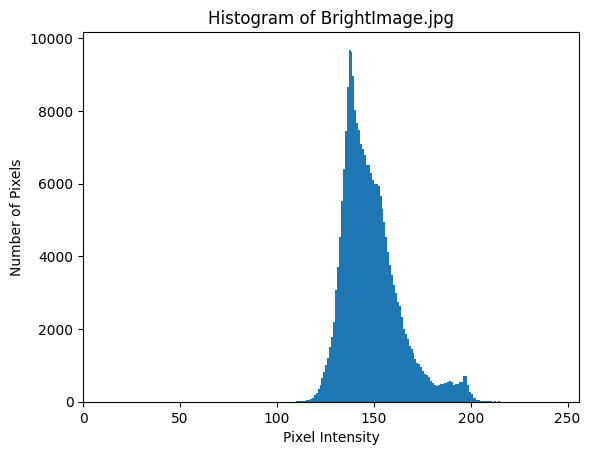
\includegraphics[width=0.85\linewidth]{images/Hist_DI_optimal.png}
    \caption{هیستوگرام متمرکز \texttt{DarkImage}}
\end{subfigure}

\vspace{0.5cm}

% سطر دوم: تصویر و هیستوگرام روشن
\begin{subfigure}{0.48\textwidth}
    \centering
    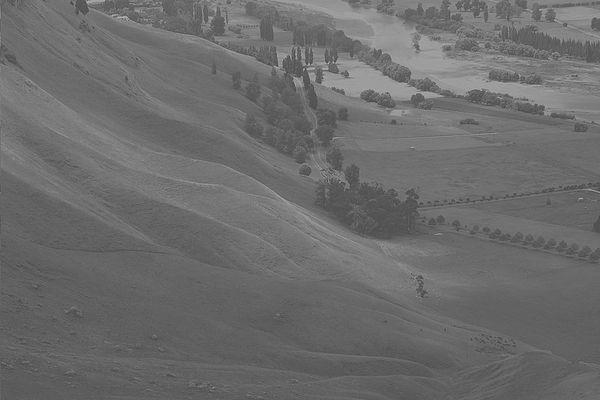
\includegraphics[width=0.85\linewidth]{images/I_BI+b_BI.jpg}
    \caption{تصویر \texttt{BrightImage} بهینه‌شده}
\end{subfigure}
\hfill
\begin{subfigure}{0.48\textwidth}
    \centering
    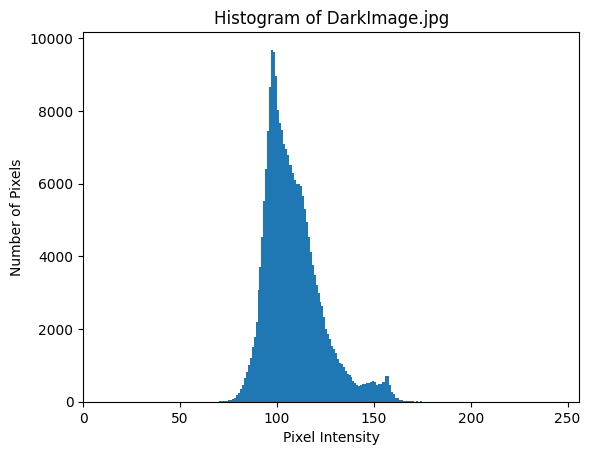
\includegraphics[width=0.85\linewidth]{images/Hist_BI_optimal.png}
    \caption{هیستوگرام متمرکز \texttt{BrightImage}}
\end{subfigure}
\caption{نتایج حاصل از اعمال شیفت تطبیقی بهینه؛ همان‌طور که مشاهده می‌شود، هیستوگرام‌ها به شکل متوازنی حول محدوده‌ی خاکستری (مقدار $128$) شیفت پیدا کرده‌اند.}
\label{fig:optimal_results}
\end{figure}

\begin{notebox}[نتیجه‌گیری بخش اول]
برخلاف مقادیر ثابت که کاملاً وابسته به مشاهده‌ی چشمی و آزمون‌وخطا هستند، استفاده از پارامترهای آماری هیستوگرام (مانند میانگین)، رویکردی تطبیقی ارائه می‌دهد که به‌طور خودکار تصویر را به سمت تعادل نوری هدایت می‌کند.
\end{notebox}